\chapter{TECNOLOGIAS EMPREGADAS}
\thispagestyle{empty}

Este capítulo apresenta um conceito simplifica sobre cada ferramenta utilizada para o desenvolvimento desta aplicação, ou que utilize a mesma.

\section{Python}

Python é uma linguagem de programação poderosa e fácil de aprender. Tem estruturas eficientes e de alto nível de dados além de uma abordagem simples, entretanto eficaz para programação orientada a objeto. Sua sintaxe elegante, de tipagem dinâmica, juntamente com a sua natureza interpretada, tornam-na uma linguagem ideal para \textit{scripts} e desenvolvimento rápido de aplicações em muitas áreas, na maioria das plataformas \cite{GUIDO}.

\subsection{Buildout}
\label{buildout}

\textit{Buildout} é uma ferramenta desenvolvida em python, capaz de criar um ambiente isolado para desenvolvimento de novas aplicações. Ele fornece suporte para criação diversas aplicações, especialmente em Python, mas não somente. Fornece ainda ferramentas para montagem de receitas para aplicações de múltiplas partes. Uma única aplicação pode conter vários programas, processos e definições de configuração \cite{BRANDOM}.

Levando em consideração o ideal do ambiente separado, também chamado de puro, a instalação do \textit{buildout} é extremamente simples a partir de um arquivo de \textit{script} python, que ao ser executado gera um segundo \textit{script} 'bin/buildout' e a partir deste toda aplicação pode ser gerada com base no arquivo de configuração como do \textit{script} \ref{codigo_buildout}:

{\singlespace
\begin{lstlisting}[caption=Exemplo de um \textit{script buildout},language=python,label={codigo_buildout}]
[buildout]
develop = .
parts = 
  xprompt
  test

[xprompt]
recipe = zc.recipe.egg:scripts
eggs = xanalogica.tumbler
interpreter = xprompt

[test]
recipe = zc.recipe.testrunner
eggs = xanalogica.tumbler
\end{lstlisting}
}

A descrição superior \textit{[buildout]} é a única realmente obrigatória para identificação de um arquivo de configuração. Na segunda linha definimos que o diretório em que o arquivo se encontra será um local de desenvolvimento da aplicação, nas três seguintes estão definidas suas partes, ou seja, a ordem em que cada parte, seja uma operação ou aplicação acoplada, será executada.

O \textit{recipe} trata-se do componente responsável pela parte a qual é citado. \textit{Egg} trata-se da opção referente as dependências de cada parte e por fim \textit{interpreter} representa ao \textit{buildout} que deseja-se um interpretador python contendo as dependências desta parte e que seja renomeado para \textit{xprompt}.

Assim com poucas especificações o \textit{script} 'bin/buildout' executa todos os passos necessários e gera uma nova aplicação através dessas especificações.

Ainda que incomum, volto a ressaltar que aplicações não desenvolvidas em python podem ter seu ambiente gerado pelo \textit{Buildout}, basta mudar algumas especificações e ter de fato o python instalado como dependência do \textit{buildout} e não da aplicação desejada.

\subsection{Subprocess}

O \textit{subprocess} é um modulo python que permite a aplicação expandir processos executados pelo \textit{shell}, ou que transmita-se informações de entrada, saída e erro de aplicações. Este módulo foi criado na intenção de substituir outros módulos e funções obsoletas, além de permitir também maior iterabilidade entre a aplicação e o sistema no qual se encontra.

{\singlespace
\begin{lstlisting}[caption=Exemplo de uso do \textit{subprocess},language=python,label={codigo_subrocess}]
>>> import subprocess
>>> subprocess.Popen('echo "Hello World!"', shell=True)
Hello World!
\end{lstlisting}
}

No código \ref{codigo_subrocess} existe um pequeno exemplo de como o \textit{subprocess} pode ser utilizado, neste exemplo ele é utilizado para acessar o \textit{shell}, como pode ser verificado no final da segunda linha em 'shell=True', e demonstrar um \textit{Hello World} através do comando \textit{echo}.

Em aplicações que utilizam outros ambientes isolados, ou seja, sem demais instalações, como citado na sessão anterior \ref{buildout}, é preferêncial que a variável \textit{shell} tenha valor \textit{false} na chamada da função a fim de usar as aplicações criadas neste ambiente,porém este é o valor padrão para esta variavél, assim não é preciso declará-lo, como por exemplo no código \ref{codigo_subprocess_convert}.

{\singlespace
\begin{lstlisting}[caption=Exemplo de uso do \textit{subprocess}com \textit{PIPE},language=python,label={codigo_subrocess_convert}]
command = ["convert", self.file, output]
stdout, stderr = Popen(command, 
                        stdout=PIPE,
                        stderr=PIPE,
                        env=self.environment
                        shell=False).communicate()
\end{lstlisting}
}

Embora tenha uma descrição um pouco mais complexa, esta figura esta representando uma chamada do \textit{subprocess} em que utiliza-se o comando \textit{convert}, utiliza-se a opção \textit{PIPE} para que, após executado, o comando retorne as mensagens de saída e erro respectivamente através das variáveis \textit{stdout} e \textit{stderr}. Além disso na chamada também utiliza-se a variável \textit{env} a fim de informar a aplicação caminhos para binários que estão em seu ambiente de desenvolvimento.

Assim sendo, o \textit{subprocess} pode ser considerado um dos melhores módulos python para trabalhar com ambientes isolados.

\subsection{Zope}
\label{zope}

Zope (Z Object Publishing Environment) é um serviço web livre de código aberto desenvolvido em python \cite{ZOPE2}.

Zope já foi considerado o responsável pela popularização o python, não existiu ferramenta em Perl que o levasse as pessoas como o Zope levou o python \cite{UDELL}, no entanto se tornou muito extenso e complexo, com alto nível de taxa de aprendizagem, sendo mais tarde ofuscado pela ferramenta Djando em questão de popularidade. 

Apesar da diminuição em sua popularidade, consequentemente em seu uso, a expansão do Zope resultou na criação de vários produtos independentes que facilitam na construção de aplicações python.

\subsubsection{Zope Interfaces}

Como citado na sessão \ref{zope}, diversos pacotes Zope foram criados individualmente com intuito de auxiliar na criação de outras aplicações python, de forma a não deixá-las muito extensas ou pesadas, entre elas a \textit{zope.interface} é uma aplicação independente escrita em python e mantida pela equipe Zope.

A \textit{zope.interface} foi criada com intuito de permitir a comunicação entre qualquer componentes externos que possuissem uma \textit{Application Programming Interface} (API). A ideia de criar uma interface para os componentes de uma aplicação é uma forma quase elegante de resolver um antigo problema de tipagens dinâmicas tratando as informações recebidas de forma genérica, a fim de renderizá-las para um tratamento mais específico.

\section{XML}

O \textit{Extensible Markup Language} (XML) é uma linguagem em formato de texto simples para representação de informações sobre estruturas: documentos, dados, configurações, livros, transações, faturas entre outros. Foi derivada de um formato antigo chamado SGML (ISO 8879), para ser mais flexível ao uso Web \cite{W3C-XML}.

Atualmente se tornou um dos formatos mais comuns para compartilhamento de informações em aplicações web, por ser simples de ser escrito e corresponder a um padrão comum ao HTML, que por muitos anos já vem sendo utilizado pelas mesmas.

Além disso este formato dispõe de outras vantagens como: padrão de \textit{markup}, cujo o nome é detalhado de forma redundante; a descrição da estrutura de forma geral também permite uma compreensão de código bem literal, como se fossem textos; todas suas versões são capazes de processar e ler qualquer documento XML, mesmo que algumas delas procurem por \textit{markups} específicos.

\section{Formato Aberto}

O formato aberto é uma especificação publicada para armazenar dados digitais, mantido geralmente por uma organização de padrões não proprietária, e livre de limitações legais no uso.

Um formato aberto deve ser tanto implementável em software proprietário quanto software livre, usando as licenças tipicas de cada um. Em contraste com o formato proprietário que é controlado e defendido por interesses particulares de empresas proprietárias detentoras de seus direitos.

O objetivo principal dos formatos abertos é garantir o acesso a longo prazo aos dados sem incertezas atuais ou futuras no que diz respeito às diretas legais ou à especificação técnica. Um objetivo secundário dos formatos abertos é permitir a competição, em vez de permitir que o controle de um distribuidor sobre um formato proprietário iniba o uso de um produto de competição.

\subsection{Formatos abertos de Documentos}

Embora não seja considerado o formato ideal para documentos uma vez que não possui opções de formatação; tais como itálico e negrito, o \textit{.txt} é o formato aberto mais comum para arquivos de texto por ser pequeno e na maioria dos casos dispor de vários programas de edição em qualquer plataforma operacional.

Em 01 de maio de 2005, surgiu o \textit{OpenDocument Format}(ODF), um conjunto de formatos para aplicações de escritório com o objetivo de padronizar os formatos abertos para documentos. Seu nome original era \textit{Open Document Format for Office Application}, uma iniciativa da \textit{Organization for the Advancement of Structured Information Standards}(OASIS), em cima de uma base XML criada por desenvolvedores do OpenOffice.org, responsáveis pela aplicação que na época era uma das poucas capazes de utilizar sua estrutura, senão a única.

Atualmente os formatos ODF existem a 7 anos e foram adotados por diversas aplicações, entre elas a Microsoft Office, da Microsoft, mesmo sendo um software originalmente proprietário através de um \textit{pluggin} ele permite a edição e manipulação destes formatos.

Através da figura \ref{crescimento_odf} é possível acompanhar o crescimento do uso do ODF até 2010, ano em que fez 5 anos.

\begin{figure}[ht]
    \centering
    \scalebox{0.7}{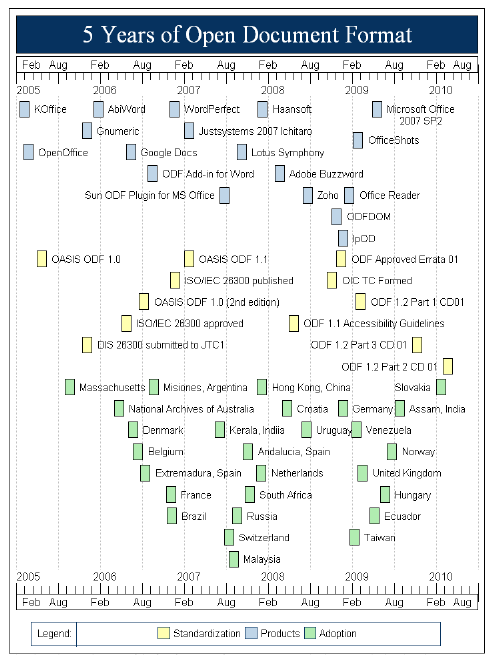
\includegraphics{figuras/crescimento_odf}}
    \caption{Crescimento do ODF nos primeiros cinco anos. Adaptado de \cite{SILVA}}
    \label{crescimento_odf}
\end{figure}

\begin{citacao}
O OpenDocument Format ainda é uma incógnita à grande maioria dos usuários comuns, mas sua adoção cresce em várias partes do mundo, especialmente nos meios corporativos e governamentais. No Brasil, por exemplo, o ODF já conta inclusive com aprovação da Associação Brasileira de Normas Técnicas (ABNT), que aconteceu em 2008 (norma NBR ISO/IEC 26300)\cite{ALECRIM-ODF}.
\end{citacao}

\subsubsection{Formatos de documentos ODF}

Embora exista um único padrão para identificação da estrutura de um ODF, como citado anteriormente, existem diversas extensões para o mesmo, como é possível observar na figura \ref{extensoes_odf}:

\begin{figure}[ht]
    \centering
    \scalebox{0.7}{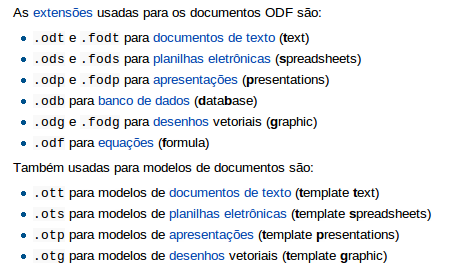
\includegraphics{figuras/extensoes_odf}}
    \caption{Extensões do ODF. Adaptado de \cite{WIKIPEDIA-ODF}}
    \label{extensoes_odf}
\end{figure}

Além destas extensões, é possível que arquivos ODF possam ainda utilizar da extensão de arquivo comprimido ZIP, outra opção de formato aberto só que para diversos arquivos a fim de diminuir seu tamanho.

\subsubsection{Estrutura de documentos ODF}

Sendo o ODF um conjunto de formatos abertos padrão, ele é constituído de uma estrutura única a fim de que toda e qualquer aplicações que o manipule obedeça seu padrão e permita que futuramente ele possa ser reutilizado por outra aplicações ou mesmo para permitir a extração de seus dados.

Esta estrutura é composta principalmente por:

\begin{itemize}
    \item{mimetype: arquivo de linha única constituído pelo mimetype do documento;}
    \item{content.xml: arquivo que armazena o conteúdo criado pelo usuário do documento;}
    \item{meta.xml: arquivo responsável por armazenar os \textit{metadados} do documento, ou seja, dados como autor, data de criação, data de modificação e outros;}
    \item{styles.xml: arquivo que contém os estilos do documento, tais como formatações de texto, parágrafos e outros;}
    \item{Pictures: pasta que armazena figuras existentes no documento.}
\end{itemize}

Existem ainda diversos arquivos e pastas que podem compor um documento ODF para compor o arquivo final, assim pode-se concluir que estes formatos representam uma diferente linha de arquivos comprimidos.

\subsection{Formatos de Imagens}

No que desrespeito a imagens a questão livre trata sobre patentes dos formatos, ou inclusa neles.

Assim em 1996 surgiu o formato \textit{Portable Network Graphics}(PNG) que tinha como principal objetivo substituir o formato GIF, portador de inúmeros algoritmos patenteados.

O PNG é um formato livre, criado desde o início para ser utilizado em qualquer aplicação sem necessidade de pagamentos de licenças ou afins.

Além disso este formato permite comprimir imagens sem perda de qualidade e também a retirada do fundo de imagens através do canal alfa; possui suporte de milhões de cores, diferentemente do GIF, cujo suporte era de 256 cores; e ainda permite a criação de animações, cujas extensões podem variar em \textit{.mng} e \textit{.apng}, mas são igualmente livres.

Este é apoiado pela \textit{World Wide Web Consortium}(W3C) e o único formato realmente livre existente no momento, e em 2003, mesmo ano em que a patente do formato GIF expirou, tornou-se padrão internacional.

\subsubsection{Estrutura do PNG}

Um arquivo PNG consiste de uma assinatura PNG e seguido de vários blocos em serie \cite{PNG-BOOK}.

Sua assinatura equivale aos primeiros oito \textit{bytes}, consiste da serie “137 80 78 71 13 10 26 10”.

Cada bloco consiste de:

\begin{itemize}
    \item{length: inteiro correspondente ao numero de \textit{bytes} dos dados da imagem;}
    \item{chunk type: código equivalente ao tipo do bloco;}
    \item{chunk data: dados da imagem;}
    \item{Cyclic Redundancy Check(CRC): campo que contém o valor total de \textit{bytes} do bloco, o \textit{chunk type} e o \textit{chunk data}, mas sem o valor do \textit{length}.}
\end{itemize}

O inicio da serie de blocos deve conter um \textit{IHDR chunk} e o ultimo bloco deve conter um \textit{IEND chunk} como \textit{chunk type} sinalizando que representam o inicio e fim da serie respectivamente.

\subsubsection{Exif}

O \textit{Exchangeable Image File Format}(Exif) é um conjunto de \textit{metadados} a respeito da imagem em questão, ou seja, são dados como autor, dia em que a foto foi tirada, câmera utilizada, entre outros listados conforme um padrão.

Todas essas informações ficam dentro da própria imagem, no entanto é preciso ter uma aplicação especifica para vê-lo, e em casos de informações mais abrangentes, as vezes é necessário possuir também uma aplicação para manipular a imagem e inserir nela \textit{metadados} a respeito da imagem.

\subsection{Formatos de Áudio}

Os formatos livres de áudio tratam sobre codecs disponíveis sem uma patente aplicada aos mesmos. Nesta categoria conta-se com os formatos de \textit{Vorbis}(OGG) e \textit{Free lossless Áudio Codec}(FLAC).

O FLAC é um formato livre de áudio comprimível e sem perda de qualidade e dados durante a o processo de compreensão. Seu algoritmo permite que o arquivo reduza em até 60\% seu tamanho original, e também permite a manipulação de \textit{metadados}.

OGG Vorbis é um novo formato comprimível de áudio É grosseiramente comparado com outros formatos utilizados para guardar e reproduzir musicas, tais como MP3, VQF, AAC, e outros formatos de áudio digital. Mas é diferente de todos estes formatos porque é livre, aberto e sem patentes \cite{XIPH}.

\subsection{Formatos de Vídeo}

Assim como os arquivos de áudio, a licença dos formatos de vídeo tratam sobre patentes de codecs, e neste caso as extensões mais comuns são conhecidas por \textit{Theora}(OGV) e \textit{Matroska}(MKV).

Theora é de proposito geral, um codec de vídeo com perda de dados. É baseado no codec de vídeo VP3 produzido pela On2 Tecnologies \cite{XIPH-THEORA}.

Matroska é o nome de uma iniciativa ousada para a criação de formatos universais de contentores, ou \textit{containers} de áudio e vídeo digitais \cite{WIKIPEDIA-MATROSKA}.

Assim o MKV trata-se de um contentor de padrão aberto para vídeos, que pode conter vários dados de diferentes tipos de codificações.

\section{LibreOffice}

O LibreOffice é um pacote de software de produtividade compatível com a maioria dos softwares semelhantes, e esta disponível para varias plataformas. Ele é um software de código aberto e, por isso, é livre para baixar, utilizar e distribuir \cite{LibreOffice}.

Este pacote teve inicio em 2000, quando a Sun Microsystems liberou o código de seu produto StarOffice, e se chamava OpenOffice.org. Em 2010 a comunidade que desenvolvia o projeto anunciou a fundação independente \textit{The Document Foundation}, a fim de cumprir com a independência explicita da carta de inicio do projeto.

Assim no inicio de 2011 foi lançado o LibreOffice 3.3, que bem como o OpenOffice.org 2.0, já suportava a edição da suíte \textit{OpenDocument}.

\subsection{UNO}
\label{uno}

O projeto OpenOffice.org possui uma característica muito útil e pouco utilizada que é a capacidade de integrar seu funcionamento com outros aplicativos. Isto é possível através do UNO (Universal Network Objects), que é um modelo de componentes do OpenOffice.org.

O UNO oferece interoperabilidade entre diferentes linguagens de programação, diferentes modelos de objetos, diferentes arquiteturas e processos, em uma rede local ou mesmo através da internet. Seus componentes podem ser implementados e acessados por qualquer linguagem de programação que possua acesso aos \textit{bindings} do UNO \cite{MINETTO-PYUNO}.

Atualmente existem \textit{bindings} para as linguagens C, C++, Java e Python. Desde a versão 1.1 o OpenOffice.org dispõe do pyUNO em sua instalação por padrão.

\subsubsection{PyUNO}

O PyUNO representa uma ``ponte'' entre o LibreOffice e aplicações Python. Através dele é possível a manipulação do componente UNO, seção \ref{uno}, para utilizar praticamente todas funcionalidades disponíveis no LibreOffice por \textit{scripts} Python.

No entanto, segundo \cite{PYUNO}, essa ferramenta ainda não atingiu seu uso absoluto podendo conter diversos \textit{bugs}, e assim dependendo em grande parte de coloboração por parte da comunidade que utiliza a mesma.

Na Figura \ref{exemple_uno} é possível ver um exemplo pratico do uso do PyUNO em um código python:

\begin{figure}[ht]
    \centering
    \scalebox{0.7}{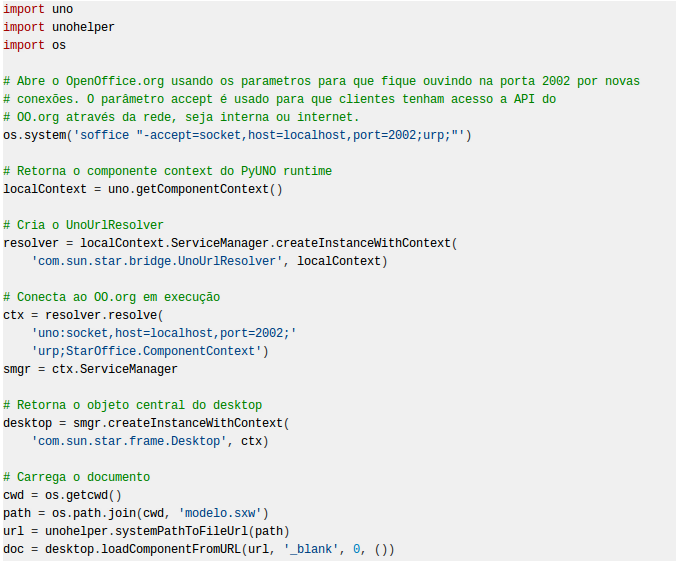
\includegraphics{figuras/exemple_uno}}
    \caption{Exemplo de uso do UNO com python(PyUNO). Adaptado de \cite{MINETTO-PYUNO}}
    \label{exemple_uno}
\end{figure}

Nela é possível observar passo a passo o código python, atentando aos comentários, neste exemplo ele utiliza o LibreOffice em \textit{localhost}, ou seja, suas modificações são apenas realizadas na própria maquina, no entanto, no caso de um serviço web é possível passar o endereço do mesmo e alterar a porta utilizada para estabelecer comunicação.

\section{ImageMagick}

ImageMagick é uma suíte de aplicações para criar, editar,compor ou converter imagens \textit{bitmap} \cite{IMAGEMAGICK-STUDIO}.
Na realidade o ImageMagick disponibiliza um conjunto de binários, compatíveis com varias plataformas, que no Linux são dados como comandos separados para diversas funcionalidades.

Para \cite{TESLA} é uma ferramenta, originalmente criada por John Cristy, para visualizar e manipular imagens, que esta amplamente disponível na Internet.

As funcionalidades que podem ser consideradas mais comuns e utilizadas são \textit{convert} e \textit{identify}, essas funcionalidades podem respectivamente: converter imagens para outros formatos ou formatação, como invertido ou de girar em 180 graus; e identificar os \textit{metadados} disponíveis na imagem, como autor, ou data que foi criada ou tirada.

\section{XPDF}

Xpdf é uma ferramente de código aberto para visualização de arquivos Portable Document Format(PDF) \cite{GLYPH-COG}.

Além de permitir a visualização de arquivos PDF o \textit{xpdf} é uma ferramenta que permite a extração de textos dentro destes formatos de arquivos e a conversão dos mesmos para \textit{postscript}, formato de arquivos especialmente compostos de informações e desenvolvido originalmente pela \textit{Adobe System}.

Assim como a maioria das aplicações para Linux é utilizada através de comandos, neste caso o mais comum \textit{pdftotext} o qual captura o texto disponível no arquivo PDF e passa para aplicação que o utilizou em forma de texto simples.

\subsection{Poppler}

O poppler é uma biblioteca para renderizar PDF baseada no xpdf 3.0 \cite{JOHNSON}.

É uma das bibliotecas de código livre mais utilizada pelos sistemas Linux para leitores PDF, seu desenvolvimento é idealizado pela FreeDesktop.Org.

\section{PDFTk}

Se o PDF é um trabalho eletrônico, então o pdftk é o removedor de grampo, furador, pasta, anel decodificador secreto e o óculos de raio-X. Pdftk é a ferramenta simples para fazer as tarefas de todos os dias com documentos PDF \cite{STEWARD}.

Esta ferramente esta sob licença GPL e utiliza bibliotecas que possuem suas próprias licenças de uso.

Na realidade de simples o \textit{pdftk} tem apenas seu uso, é uma ferramenta de fácil utilização, que no entanto permite a livre manipulação de documentos PDF, criado pelo autor do livro “PDF Hacks”, Sid Steward, é considerada uma ferramenta profissional.

\section{FFMPEG}

Para \cite{FFMPEG-SCALABLE}, a melhoria constante do uso do processamento de multimédia, requerida e obtida pela expansão multifuncional e acelerada dos equipamentos de hardware, requer também aplicações eficientes e escaláveis a medida que este processo avança. E partindo deste principio uma das ferramentas ideias para projetos escaláveis é o FFMPEG.

Ffmpeg é um rápido conversor de vídeo e áudio que também consegue tratar informações momentâneas de ambos. Ele também pode converter faixas arbitrarias de amostras e redimensionar vídeos através de filtros polifásicos de alta qualidade \cite{FFMPEG}.

Mais do que isso, o \textit{ffmpeg} é uma suíte de aplicações via linha de comando capaz de converter, extrair e inserir \textit{metadados} em arquivos de áudio e vídeo de simples entendimento, de fácil uso.

\section{SERVIÇOS WEB}

Segundo \cite{Pirnau-Apetrei-Badea}, os serviços web representam a metodologia em que aplicações podem se comunicar através de mensagens assíncronas ou chamadas remotas. Assim pode se dizer que serviços web são aplicações acessáveis remotamente.

Toda empresa tem por objetivo prover serviços, sejam esses para própria empresa, ou para clientes, que por sua podem ser outras empresas. A anos esses serviços têm sido automatizados, inicialmente aplicações \textit{desktop} eram criadas quando a empresa era pequena e possui poucas maquinas, ou a comunicação entre elas não era tão necessária.

Quando a rede passou a estar presente no dia a dia de forma geral essas aplicações foram evoluindo e buscando a comunicação entre as mesmas.

Este conceito na verdade trata da iniciativa por parte dessas empresas de retirar suas aplicações da maquinas próprias e passá-las para potente servidores que disponibilizarão esta na internet, assim basta ter acesso a internet e é possível utilizar esta aplicação.

\section{XML-RPC}

É um protocolo para chamadas remotas que utiliza HTTP para transporte e XML para encodificação. O XML-RPC foi desenhado para ser o mais simples o possível, enquanto permite que uma estrutura de dados complexa seja transmitida, processada e retornada \cite{XMLRPC}.

Foi originalmente criado por Dave Winer na UserLand Frontier, e inspirado por outros dois protocolos, um também desenvolvido pelo próprio Dave Winer e outro que representava o começo do protocolo SOAP. Entretanto seu uso é bem mais simples de se utilizar e entender que o SOAP. Suas mensagens correspondem a uma requisição HTTP-POST, enquanto composição do corpo da mensagem é escrita em XML, bem como a resposta que a requisição recebe.

\section{WSGI}

O \textit{Web Service Gateway Interface}(WSGI) é uma Interface de entrada para serviços web. É uma especificação para serviços e aplicações web para que haja comunicação com outras aplicações web(embora possa ser utilizada para outras funções). É um padrão Python, escrito sob a PEP 333 \cite{WSGI}.

Esta interface foi escrita com o objetivo de fornecer uma forma relativamente simples e compreensiva de comunicação entre aplicações e servidores, ou pelo menos com a maioria das aplicações web em python, e que ainda pudesse suportar componentes \textit{middleware}.

\subsection{Paster}

O \textit{Paster} se trata de um servidor web, composto pelo \textit{Python Paste}, que segue o padrão da interface python WSGI.

Possui dois níveis de linha de comando composto inicialmente por \textit{paster}, onde o segundo comando especifica o serviço desejado, como \textit{serve} no caso de estabelecer o servidor, seguindo como parâmetros o restante das informações necessárias para estabelecer o serviço desejado.

É considerado um dos mais simples servidores web para python, no entanto pode ser utilizado assincronamente e manter uma escalabilidade considerável até 2000\textit{rps}.

\section{Git}

Git é um sistema de controle de versão distribuída livre e de código aberto, projetado para lidar com qualquer projeto, desde o menor ao maior com rapidez e eficiência \cite{SOFTWARE-FREEDOM-CONSERVANCY}.

A historia do Git está muito relacionada a criação do Linux e de seu criador Linus Torvalds, bem como com toda comunidade de desenvolvimento Linux. Durante anos a comunidade utilizou a ferramenta \textit{BitKeeper} para guardar a modificações do projeto.

Em 2005, após um problema com a proprietária deste, a comunidade decidiu criar sua própria ferramenta a partir da experiencia com a anterior, houve um novo foco em: velocidade, \textit{design} simples, suporte para desenvolvimento paralelo, distribuição completa e a habilidade necessária para lidar com projetos grandes sem perda de velocidade e dados.

Assim, esse novo sistema de versionamento permite que qualquer repositório seja o centro do versionamento, deixando todo \textit{log} das modificações guardados nele sem que para isso precise de uma conexão a rede ou servidor geral.

\subsection{Git e Subversion}

Diferentemente do \textit{git}, o \textit{subversion} é um sistema de controle de versões centralizado, ainda muito utilizado atualmente, principalmente por projetos livres.

Embora seja consideravelmente rápido, é extremamente desaconselhável para projetos grandes e principalmente desenvolvidos paralelamente.

\subsection{Biblioteca Digital}

A Biblioteca Digital da Rede Nacional de Pesquisa e Inovação(RENAPI), é um projeto que visa disponibilizar um acervo bibliográfico digital para contribuir com a disseminação de material científico e tecnológico produzido na rede de Educação Profissional Científica e Tecnológica(EPCT), sendo esse material periódicos, teses, monografias, artigos entre outros. Assim esse disseminação visa colaborar na qualificação do material humano digitalizado e na disseminação de conhecimento.

Este projeto é um dos principais desenvolvidos no Núcleo de Pesquisa em Sistemas de Informação(NSI), que conta atualmente com ??? bolsistas e ??? pesquisadores.

\subsection{ERP5}

Um ERP é capaz de integrar processos e dados de uma organização, através de recursos tecnológicos que padronizam e automatizam os mesmos.

Muito seja um sistema propriamente dito, ele foca mais em processos do que em funcionalidades, ele mascará informações em funcionalidades transparentes(\cite{PITRE-DESAI}).

No entanto, apesar de trazer muitas vantagens a organização, esse processo de automatização, de forma geral, é longo, de alto custo e complexidade, e até mesmo difícil de implementar.

De acordo com \cite{SMETS-CARVALHO}, esta situação que motivou a criação do ERP5, cujas ferramentas são de código aberto, permitindo que a organização modifique-o a fim de torná-lo mais flexível aos seus processos.

Ele também incorpora conceitos avançados como o de banco de dados orientados a objetos, um sistema de gerenciamento, de sincronização, variação, \textit{workflows}, e possibilita a implementação de \textit{Business Templates}.

Compreende-se assim o ERP5, como sendo um ERP de baixo custo de implantação e alta tecnologia para pequenas e médias empresas.

\subsection{SlapOS}

O SlapOS é um sistema operacional de código aberto para o uso de redes distribuídas em computação em nuvem, que se baseia em que tudo se trata de um processo.

Para \cite{SMETS-CERIN-COURTEAUD} a computação em nuvem é dividida em três camadas, infra-estrutura como serviço (IaaS), Plataforma como Serviço (PaaS) e Software como Serviço (SaaS). Na IaaS esta o funcionamento virtual da maquina e seu armazenamento, sob o ele é construido o Paas, que funciona como coração dos serviços, como servidor e bancos de dados. Finalmente sobre Paas estão as aplicações de uso do usuário.

Através de uma API unificada e simples, que requer poucos minutos para aprendizagem, este sistema combina computação em grade e o conceito de ERP para fornecer estas categorias previstas na compução em nuvem.

Dada sua abordagem unificada e arquitetura modular, ele tem sido usado como uma ferramenta de testes para benchmark de bancos de dados NoSQL e para otimização do processo de alocação em nuvem.

